\documentclass[11pt,a4paper]{article}
\usepackage[utf8]{inputenc}
\usepackage[francais]{babel}
\usepackage[T1]{fontenc}
\usepackage{amsmath}
\usepackage{amsfonts}
\usepackage{amssymb}
\usepackage{listings}
\usepackage{graphicx}


% "define" Scala
\lstdefinelanguage{scala}{
  morekeywords={abstract,case,catch,class,def,%
    do,else,extends,false,final,finally,%
    for,if,implicit,import,match,mixin,%
    new,null,object,override,package,%
    private,protected,requires,return,sealed,%
    super,this,throw,trait,true,try,%
    type,val,var,while,with,yield},
  otherkeywords={=>,<-,<\%,<:,>:,\#,@},
  sensitive=true,
  morecomment=[l]{//},
  morecomment=[n]{/*}{*/},
  morestring=[b]",
  morestring=[b]',
  morestring=[b]"""
}


\usepackage{color}
\definecolor{dkgreen}{rgb}{0,0.6,0}
\definecolor{gray}{rgb}{0.5,0.5,0.5}
\definecolor{mauve}{rgb}{0.58,0,0.82}
 
% Default settings for code listings
\lstset{frame=tb,
  language=scala,
  aboveskip=3mm,
  belowskip=3mm,
  showstringspaces=false,
  columns=flexible,
  basicstyle={\small\ttfamily},
  numbers=left,
  numberstyle=\tiny\color{black},
  keywordstyle=\color{blue},
  commentstyle=\color{dkgreen},
  stringstyle=\color{mauve},
  frame=single,
  breaklines=true,
  breakatwhitespace=true,
  tabsize=3
}

\title{Projet d'option GSI Vivaldi \\ Cahier d'Analyse et de Conception}
\author{Nicolas Joseph, Raphaël Gaschignard\\ Guillaume Blondeau, Cyprien Quilici, Jacob Tardieu}

\begin{document}
\maketitle
Ce cahier d’analyse et de conception est un document qui décrit l’architecture du projet, sa décomposition en tâches ainsi que les différentes échéances et choix technologiques que nous avons fait.
\section{Dates clés}

\begin{itemize}
\item Définition des interfaces: Samedi 16/11/2013
\item Implémentation de la version alpha: 10/12/2013
\item Début du travail sur le déploiement et des tests sur grid’5000 : 10/12/2013
\end{itemize}

\section{Architecture Logicielle du projet}
\subsection{Les différentes couches logicielles} \label{coucheslogicielles}
Nous avons choisi de diviser l’ensemble du projet en 2 couches logicielles réparties sur 3 briques :

\begin{verbatim}
|===========================Vivaldi===========================|
|                                                             |
|               ---------------------------------             |
|               |        API Utilisateur        |             |
|-------------------------------------------------------------|
|     	Communication Réseau    	|        Vivaldi-Core         |
|=============================================================|
\end{verbatim}

\subsubsection{Vivaldi Core}
Cette partie contient l’algorithme vivaldi ainsi que les variables à maintenir (tableaux des plus proches voisins et RPS : Random Preloaded Subsets, ID, coordonnées dans vivaldi).\\

Vivaldi-core récupère n (à définir empiriquement) pings effectués par la couche réseau à chaque mise à jour du tableau de RPS et ajuste sa position dans l’espace de coordonnées vivaldi par rapport à eux.

\subsubsection{Réseau}
Cette partie contient la routine de maintien des RPS\\

Toutes les m (à définir empiriquement) secondes, la couche réseau lance une routine de mise à jour des RPS. Elle se connecte alors successivement à l (à définir) noeuds de son tableau de RPS et met à jour son tableau avec un mélange des deux tableaux du noeud courant et de son interlocuteur. \\

\emph{Note:} à chaque fois, le noeud envoyant la requête de mise à jour du RPS envoie son ID dans le RPS de l’autre noeud pour maintenir l’information qu’il est dans le réseau. Un noeud est donc supprimé de l’union des deux tableaux.\\

\begin{verbatim}
|-------------|                                 |----------------|
|   Sender    |                                 |    Receiver    |
|-------------|                                 |----------------|
| Tab voisins |              réseau             |  fait new tab  |
|  *tab RPS   | ------------------------------->|     voisin     |
|-------------|                                 |   pour sender  |
                                                |----------------|
                                                        ||
                                                        ||
                                                        \/
|-------------|                                 |----------------|
|   new tab   |<--------------------------------|  merge les RPS |
|   voisins   |                                 |----------------|
|-------------|

\end{verbatim}
\subsubsection{API}
Voici les différentes fonctions qui sont à implémenter dans l’API :

\begin{lstlisting}[language=scala]
nextNode(origin: Node): Node
// Renvoie le noeud le plus proche du noeud origin passe en parametre.

nextNode(origin: Node, excluded: Set[Node]): Node
// Renvoie le noeud le plus proche du noeud origin passe en parametre en excluant la liste de noeuds excluded.

nextNodes(origin: Node, excluded: Set[Node], numberOfNodes: Integer): Node
// Renvoie les numberOfNodes noeds les plus proches du noeud origin en exluant la liste de noeuds excluded.
\end{lstlisting}

\subsection{Le Modèle Acteur}

Pour simplifier la division du travail et pour avoir un système plus modulaire, on se base sur le modèle acteur pour la coordination entre parties. Chaque système a son contexte d’exécution indépendant, et la communication entre chaque acteur se passe que par envoi de message (et pas par mémoire partagée ou verrous). Ceci nous permet de créer un programme modulaire et éviter toute une classe d’erreurs liée à la synchronisation.

 Dans notre cas,  on utilise la bibliothèque Akka de Scala comme infrastructure d’acteur.
\begin{figure}[h]
   \caption{\label{acteur} Modèle Acteur}
   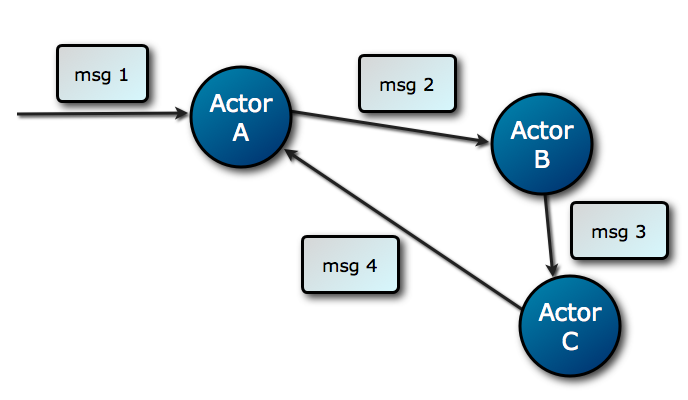
\includegraphics[scale=0.5]{acteur}
\end{figure}

\section{Organisation de l’équipe}

Le travail est divisé en plusieurs tâches. À chaque tâche est assignée un lead et un assistant. Le lead se charge de la majorité du travail de programmation alors que l’assistant aide le lead quand celui-ci en a besoin et s’occupe du “code review”. 

\subsection{Définition des tâches}
\begin{itemize}
\item Vivaldi-core
\item Réseau
\item API
\item Initialisation système: écriture de la routine d’insertion dans le réseau (créations des tableaux des plus proches voisins et RPS, propagation de son identifiant, localisation dans vivaldi).
\item Intégration: intégration de l’algorithme de vivaldi dans la structure logicielle existante (AkkaArc)
\end{itemize}

\subsection{Répartition des tâches}
\begin{tabular}{|c|c|c|c|c|c|}
  \hline
  & Vivaldi-core & Réseau & Initialisation Système & API & Intégration \\
  \hline
  Lead & Cyprien & Raphael & Guillaume & Nicolas & Jacob \\
  \hline
  Assistant & Nicolas & Guillaume & Jacob & Cyprien & Raphael \\
  \hline
\end{tabular}


\end{document}
